\section{Introduction}
Robot Programming is the process of defining desired motions and associated skills so that the robot may perform them without human intervention.
Classical robot programming processes in the industry have task-specific definitions, which are generally robot-dependent, and require programming expertise.
\fig{fig:Classical robot programming process} shows the classical robot programming process, consisting of at least four phases:
The initial task definition is followed by sequencing the workcell operations.
Once the process has been validated, the robot is programmed offline using a native programming language, before it is pushed into production for regular execution.
The programmed robot can only be used for this specific task in this particular working environment.
If the task definition needs to be altered, the programming expert needs to repeat the entire programming process.
Therefore, classical robot programming processes are time-consuming and cost intensive.

\begin{figure}[ht]
	\centering
	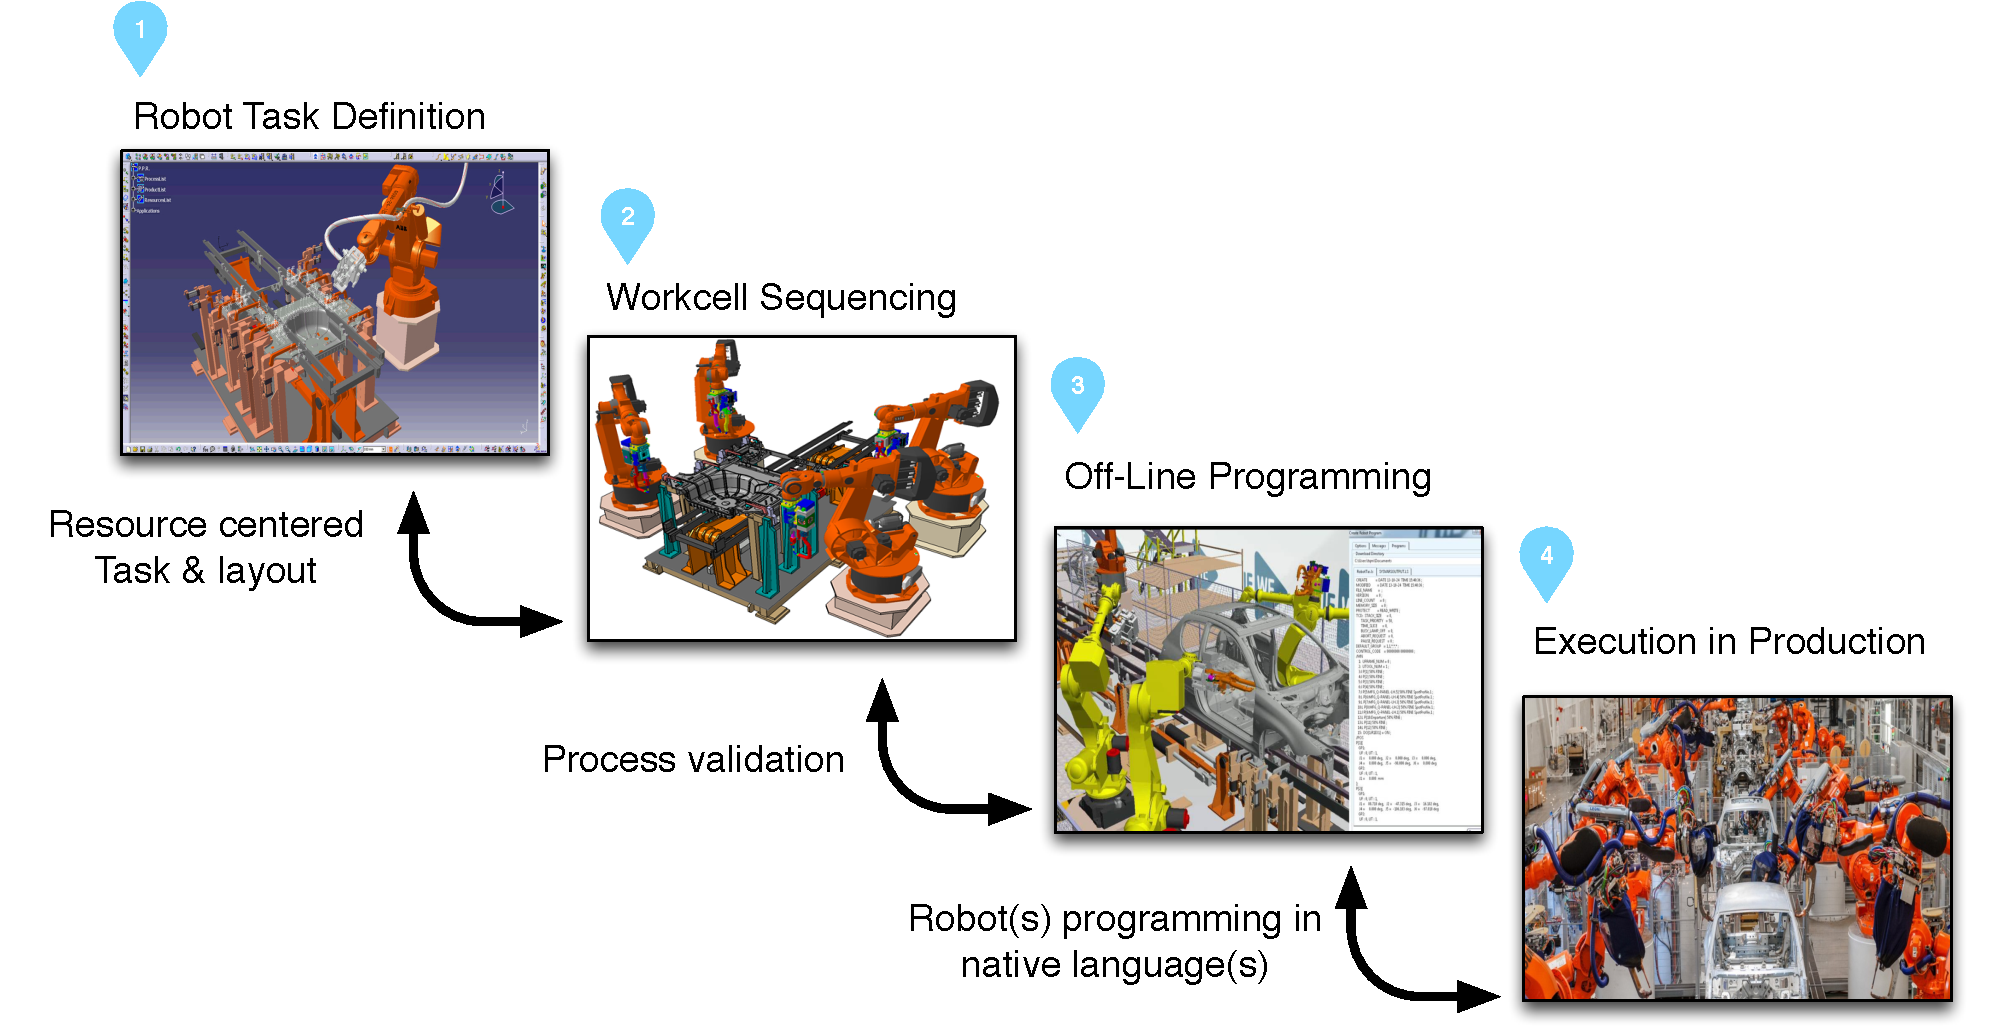
\includegraphics[width=\linewidth]{figures/manual-programming}
	\caption{Classical robot programming process}
	\label{fig:Classical robot programming process}
\end{figure}

In the past few decades, different robot programming techniques have been developed to facilitate this process. 
There are many ways to divide robot programming systems. 
\cite{lozano1983robot} divided them into three categories: 
guiding systems, where the robot's joint positions were sequentially recorded,
robot-level systems, where a programming language was used, and
task-level systems, where the task goal (\eg object positions) needs to be specified.
However, the range of programming systems was very limited at that time and examined only industrial robot programming systems.
Instead, \cite{Biggs2003} divided them into two main categories, distinguishing systems for users and for programmers:

\begin{itemize}
  \item {\textbf{Manual programming (\sect{subsec:Manual Programming Systems})}, where the user can directly control the robot's execution code, using a text-based or a graphical system.}
  \item {\textbf{Automatic programming (\sect{subsec:Automatic Programming Systems})}, where the user does not need to write explicit code and the robot learns using a learning system, Programming by demonstration (PbD), or an instructive system.}
\end{itemize}
% - also mention software architectures which are important for any robot programming systems

% \begin{figure}[ht]
% \centering
%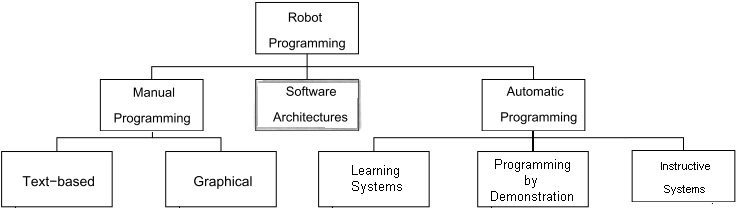
\includegraphics[width=\linewidth]{figures/Biggs2003-RobotProgramming-short}
% \caption{Robot programming categories to distinguish systems for users and programmers. (\cite{Biggs2003})}
% \label{fig:RobotProgrammingSystems}
%\end{figure} 

Inspired by \cite{Biggs2003}, we created a new robot programming overview (\fig{fig:RobotProgrammingOverview}) involving techniques that have been applied in most recent research.
Even though many state of the art systems use a combination of techniques, such as PbD for Reinforcement Learning (\cite{hester2017learning}), it makes sense to differentiate them by their key attributes.
We identified three key factors: 
%control over the robot code, learning data, and end-user involvement.
\begin{itemize}
	\item Control over the robot behaviour: if the robot behaviour code is directly entered and how it is generated (text-based or visual programming) and if the code directly encodes the robot's executed behaviour (manual or automatic programming)
	\item Learning data: for automated programming systems the robot learns from data and we differentiate how it is acquired (provided by the teacher vs by self-exploration), and what type it is (\eg positive vs negative examples, labelled)
	\item End-user involvement: the level that the end-user is involved in the programming process ranging from writing code manually, providing data or continuous feedback during the learning process to defining reward functions.
\end{itemize}

%From an end-user programming perspective, it is useful to assign different levels of teacher involvement in the programming process and an estimation of the programming time required.
In the following sections we will give a brief overview of the different programming systems by first distinguishing between the user's control over the robot behaviour, \ie manual (\sect{subsec:Manual Programming Systems}) vs. automatic (\sect{subsec:Automatic Programming Systems}) programming.
For manual programming, we compare text-based (\sect{sssec:Text-based Systems}) and graphical (\sect{sssec:Graphical systems}) systems.
For automatic programming, we differentiate those that learn from unbiased and biased data, \ie machine learning systems (\sect{sssec:Learning Systems}) vs programming by demonstration (\sect{sssec:PbD}).
Finally, we will discuss different levels of end-user involvement and their interaction modalities (\sect{sssec:End-User Involvement}).

%\begin{table}[ht]
%\begin{center}
%\begin{tabular}{r|c|c}
%Programming Techniques & by Exploration \newline (unguided) & by Demonstration \newline (guided)\\ \hline
%Classification & \checkmark & \checkmark \cite{saunders2006teaching,hovland1996skill,rybski1999interactive} \\
%Regression & \checkmark & \checkmark \cite{atkeson1997locally,pomerleau1991efficient} \\
%Reinforcement Learning & \checkmark & \checkmark (System models) \cite{atkeson1997robot,smart2002effective,abbeel2004apprenticeship}.\\
% Plans & \checkmark & \checkmark \cite{kuniyoshi1994learning,ekvall2008robot} \\
% \hline
%Human-Robot Interaction & & \\ \hline
% touch & \checkmark (learning by poking) & \checkmark \\
% vision & \checkmark & \checkmark \\ 
% voice & n/a & \checkmark (instructive, create sequence by voice) \\
%\end{tabular}
%\end{center}
%\label{tab:Programming Overview}
%\end{table}

\begin{sidewaysfigure}
	\centering
	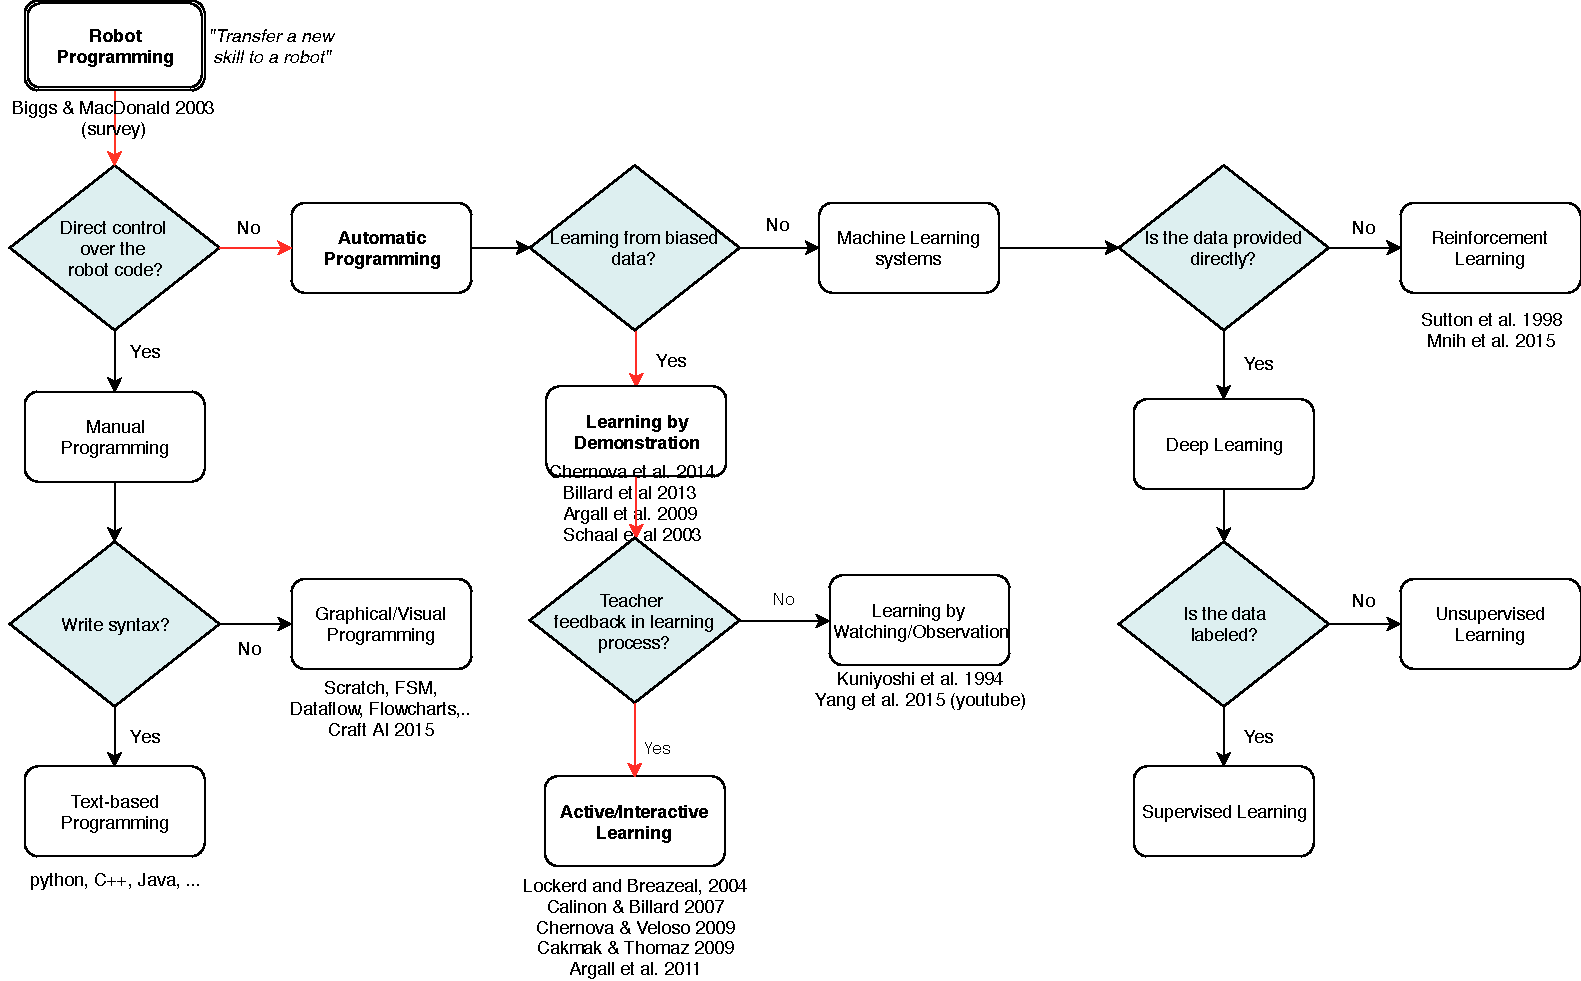
\includegraphics[width=\linewidth]{figures/RobotProgrammingOverview}
	\caption{Overview of Robot Programming methods.}
	\label{fig:RobotProgrammingOverview}
\end{sidewaysfigure}

\newpage

\section{Manual Programming Systems}\label{subsec:Manual Programming Systems}
In manual programming systems users have direct control over the robot code
and often require expert knowledge in a programming language. % and a good understanding of the program flow.
There exist a variety of tools to make programming, as well as testing and debugging, easier such as IDEs, spreadsheets, macros, \etc
There are two types of manual programming: text-based programming, where the code is written manually in a chosen programming language (python, C++, java, \etc) and graphical programming, where the code structure is created with the help of a graphical interface (\eg Flowcharts). 

\subsection{Text-based Systems}\label{sssec:Text-based Systems}
Text-based systems are one of the most common methods and use a traditional programming approach. 
Depending on the type of language used, the user performs programming in either controller-specific languages, where the robot-specific machine language consists of simple commands, \eg the KUKA Robot Language (\cite{braumann2011parametric,muhe2010reverse}) shown in \fig{fig:Kuka},
% RAPID a high-level programming language to control ABB robots
generic procedural languages, where multi-purpose languages such as C++ that have been extended with classes to provide simple access to common robot specific functions ({\eg Lego}), or behaviour-based languages that specify how the robot should react to different conditions (\eg Haskell). 
There has been a trend to move from low-level command-based languages towards more intelligent programming systems with high-level languages that provide more support to the user and reduce the programming workload.
However, text-based systems still require trained users with programming knowledge and are more likely to be used by robot developers than end-users.

\begin{figure}[!h]
	\centering
	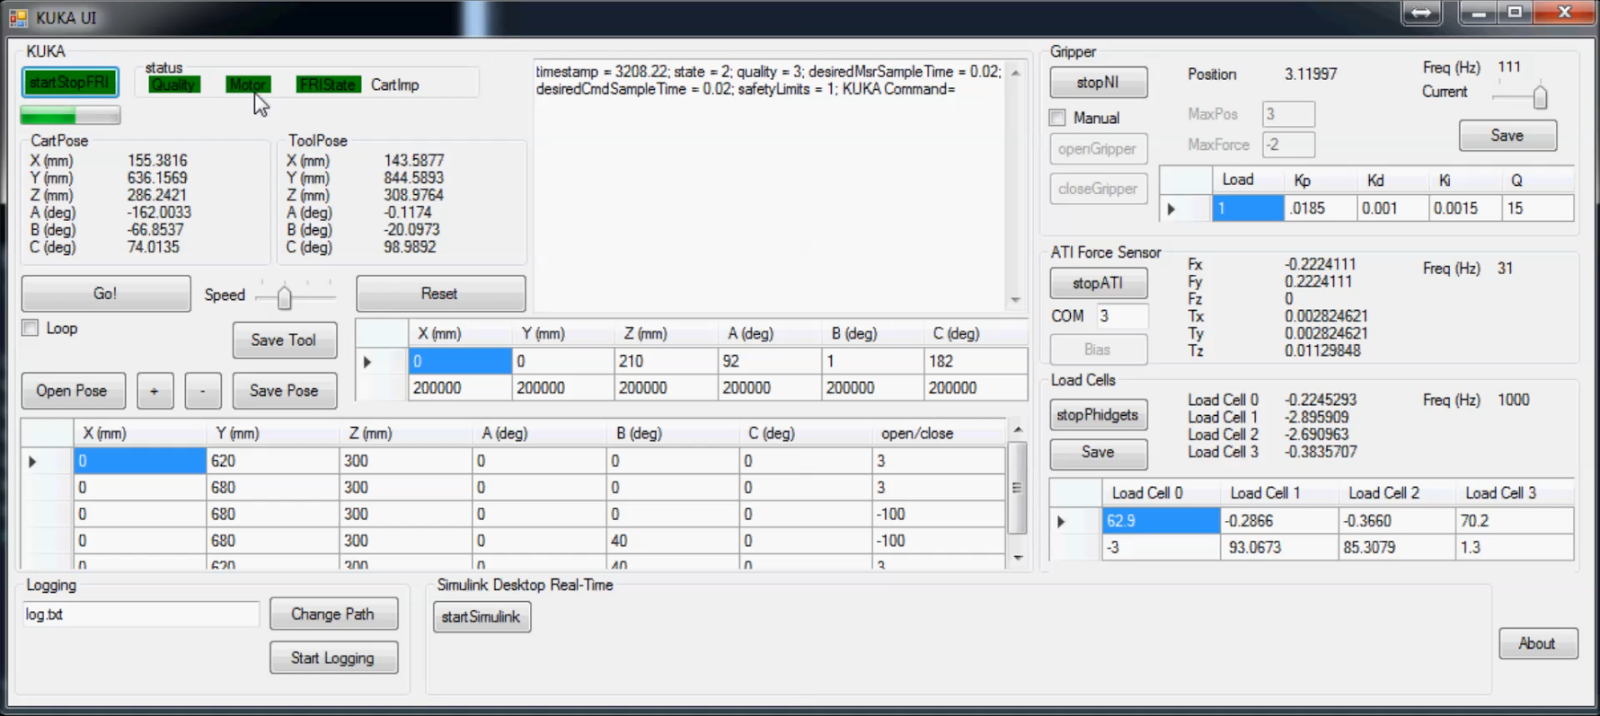
\includegraphics[width=\linewidth]{figures/kuka-interface2}
	\caption{KUKA Robotics graphical user interface (\cite{abdeetedal2017kuka})}
	\label{fig:Kuka}
\end{figure} 
\begin{figure}[!h]
\centering
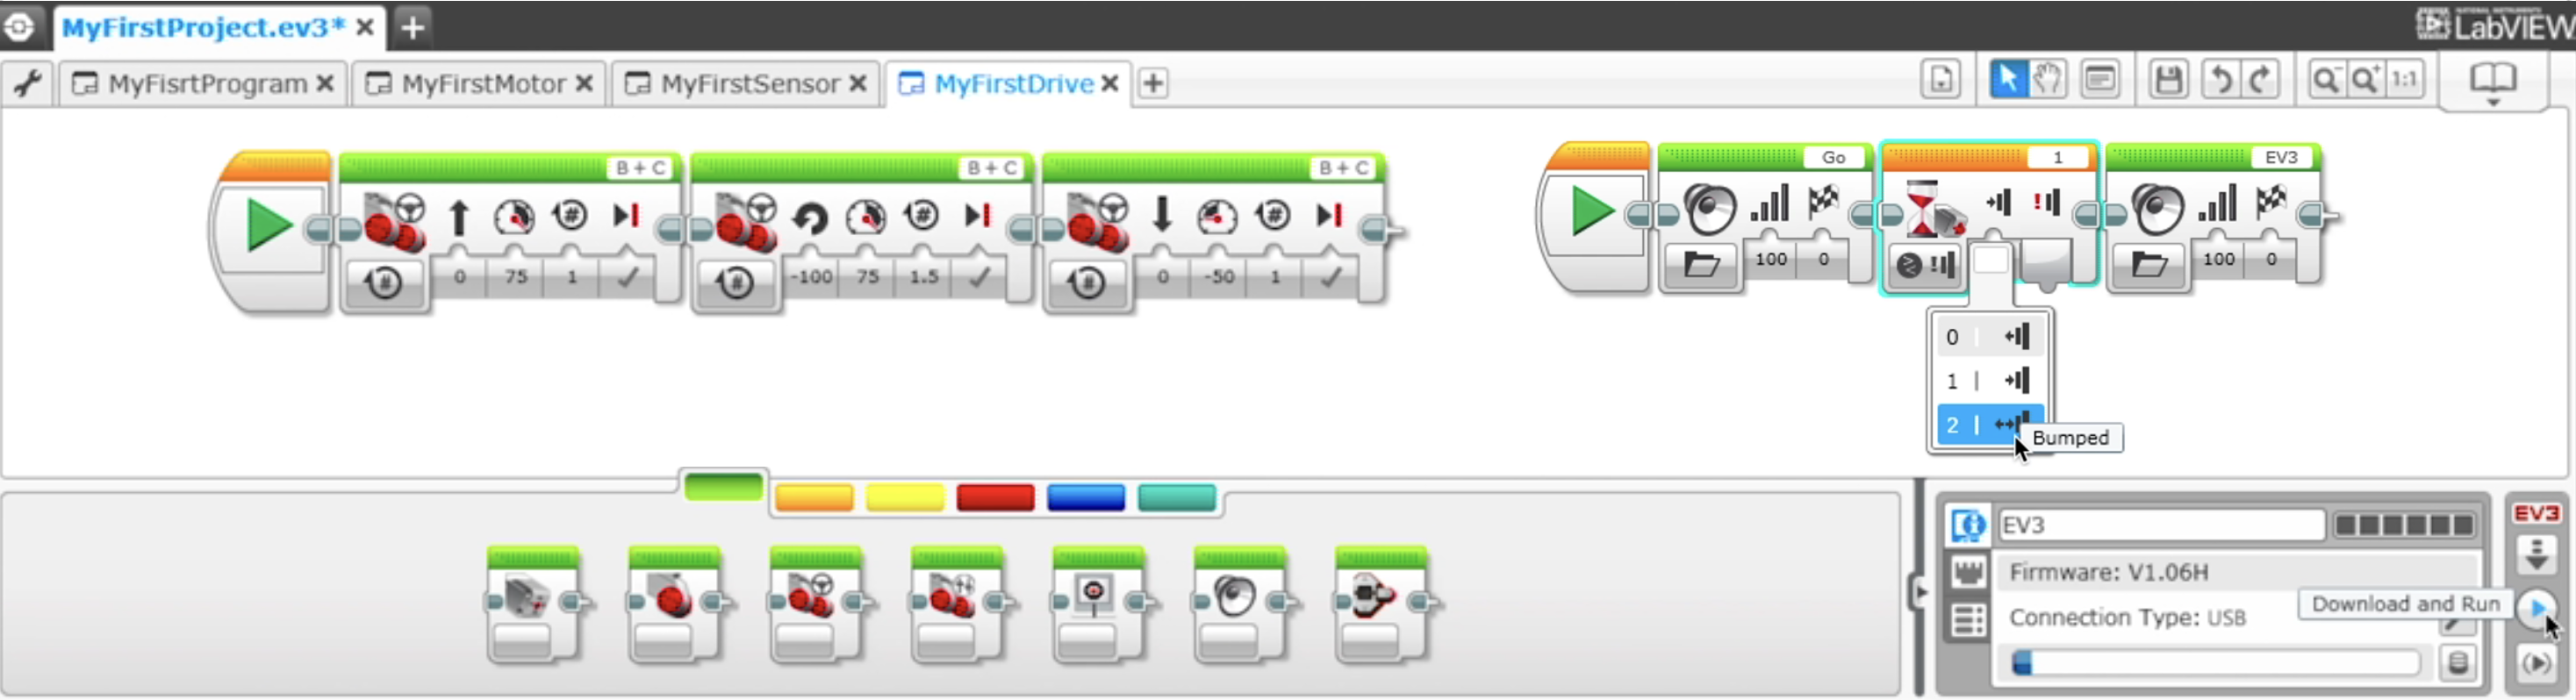
\includegraphics[width=\linewidth]{figures/lego-mindstorm2}
\caption{Lego Mindstorms EV3 icon-based interface (\cite{lego2003})}
\label{fig:lego-mindstorm}
\end{figure} 
\begin{figure}[h]
	\centering
	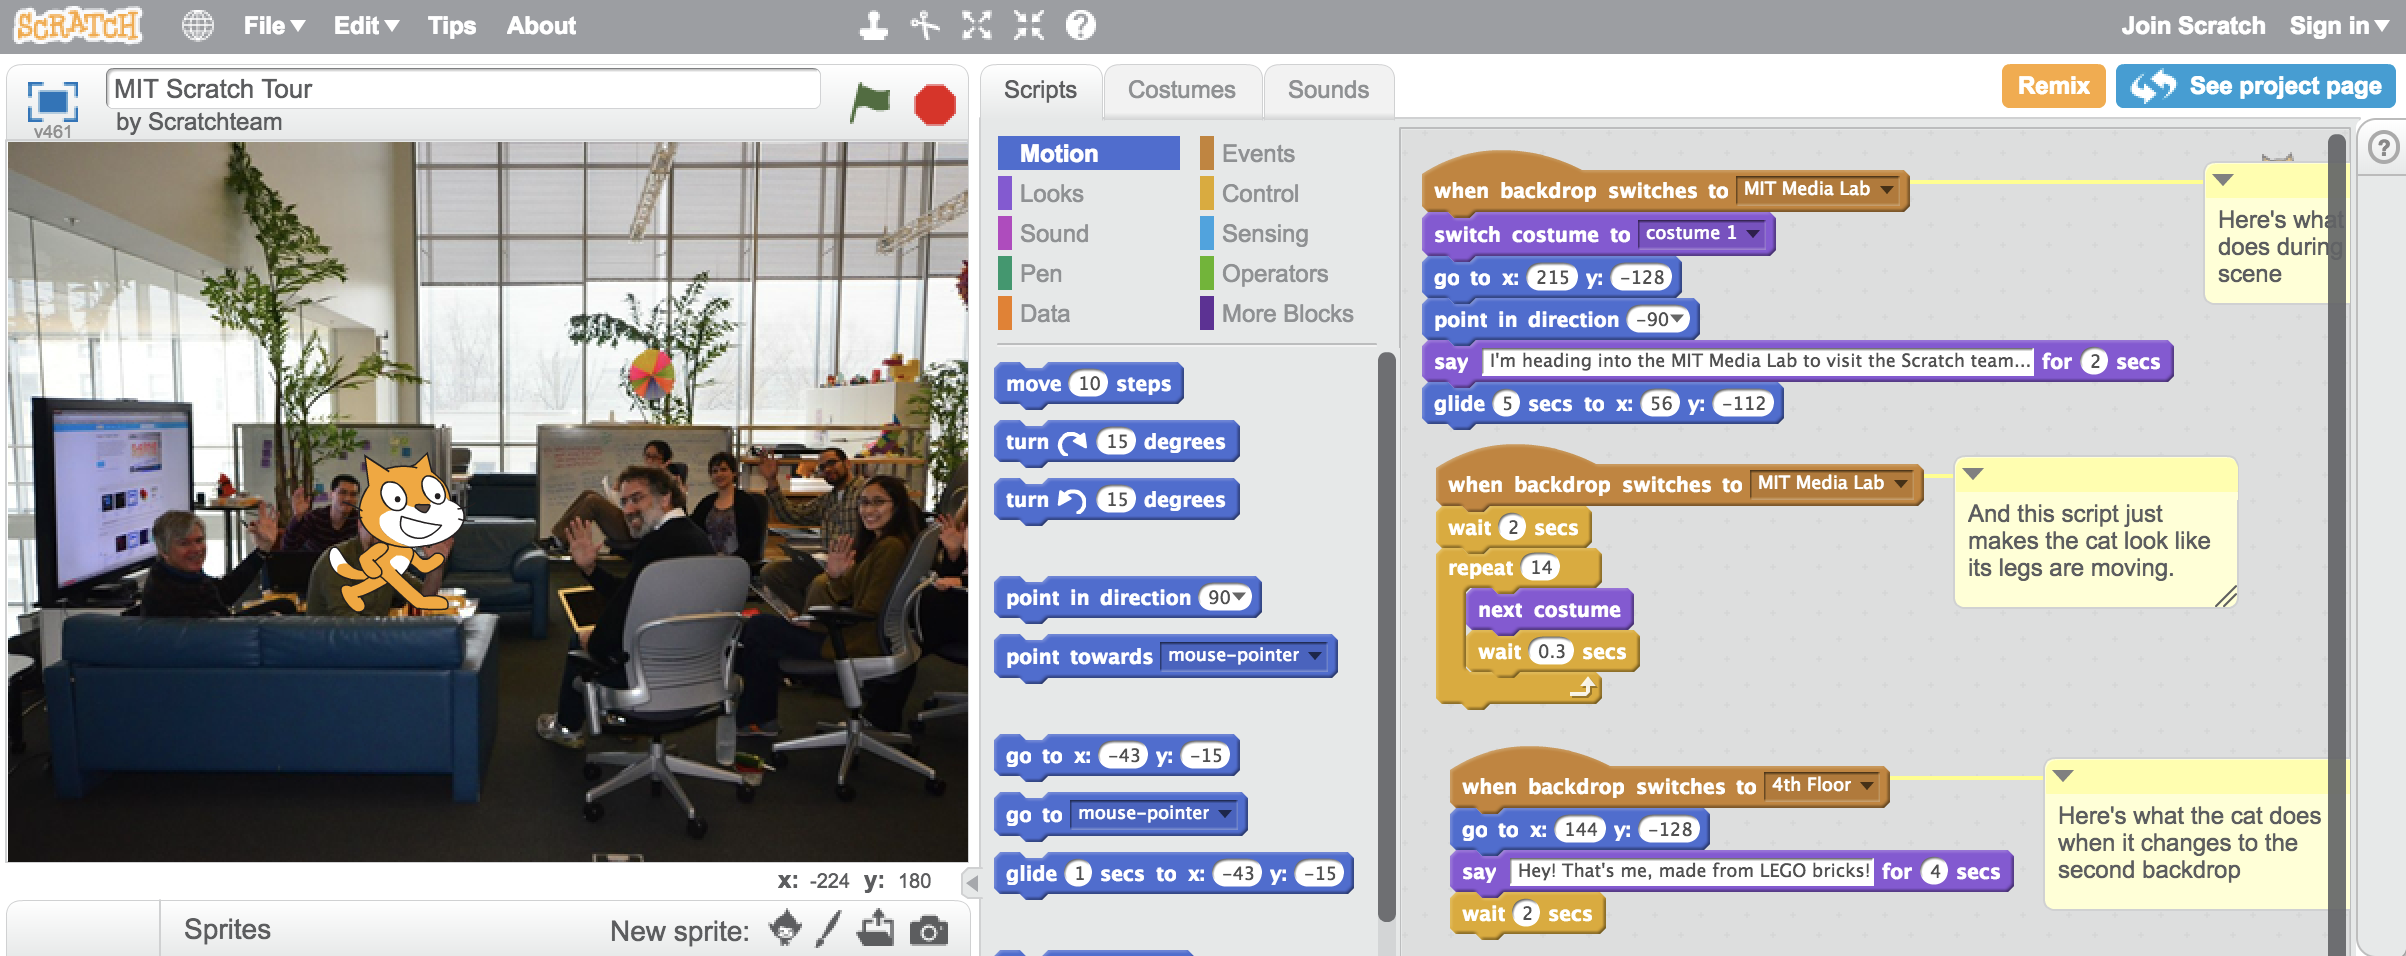
\includegraphics[width=\linewidth]{figures/scratch-interface}
	\caption{Scratch: block-based visual programming language (\cite{majed2014learn})}
	\label{fig:scratch-interface}
\end{figure} 

\subsection{Graphical Systems}\label{sssec:Graphical systems}
Graphical (or icon-based) systems use a graph, flow-chart or diagram view where users manually specify actions and program flow.
The graphical icons correspond directly to the program statements.
\cite{lego2003} and \cite{bischoff2002morpha} produced graphical systems using a flow-chart approach, where the robot's behaviour can be configured by arranging low-level actions in a sequence (\fig{fig:lego-mindstorm}).
Similarly, Scratch (\cite{majed2014learn}) is a block-based visual programming language to allow children with no programming experience to learn development in an intuitive way \fig{fig:scratch-interface}).
They are typically easy to use and generally used for robot applications rather than system programming. 

\section{Automatic Programming Systems}\label{subsec:Automatic Programming Systems}
Automatic programming systems relate to robots that can learn from data and generate their behaviour from information entered into the system.
Unlike manual programming, the end-user does not need to sequence robot code and does not have direct control over the robot's executed behaviour.
The robot can learn from data that is directly related to the desired robot behaviour and has been selected by a teacher, we will refer to this as \textit{biased} data.
If the robot learns from data that is not directly related to its required behaviour, we refer to the data as being \textit{unbiased}.
Thus, we differentiate automatic programming systems between Machine Learning systems, where the robot learns from \textit{unbiased} data, and Programming by Demonstration, where the robot learns from \textit{biased} data in the form of demonstrations provided by the teacher.

\subsection{Machine Learning Systems}\label{sssec:Learning Systems}
Machine Learning (ML) systems use inductive inference to create a program by taking examples provided by the user or from self-exploration of the robot. 
The goal of these systems is to construct programs that allow the robot to automatically improve its performance with increasing amounts of data. 
Even though ML algorithms have been around since the 1980s, it has only become popular in the past few decades. 
The rise of the internet led to big data, improved knowledge sharing, as well as advances in techniques to process and store data efficiently lead to a wave of new ML techniques.
%Developments in various research areas such as computer vision have impacted the field of robotics.
Recent applications of ML in robotics\footnote{http://techemergence.com/machine-learning-in-robotics/} include research areas such as computer vision (or ``robot vision'') for the identification and sorting of objects (\cite{stager2013computer}) and imitation learning to learn action plans from watching unconstrained videos (\cite{Yang2015}).

We differentiate between Deep Learning systems, where the data is provided directly to the robot, and Reinforcement Learning, where the robot acquires data by exploration of its environment (\fig{fig:ml-types}).
Deep learning systems (\cite{schmidhuber2015deep}) generally use artificial neural networks (NN) with different architectures which require large amounts of data to learn the desired behaviour.
Techniques are divided into supervised (\eg Classification, Regression) and unsupervised (\eg Clustering) learning, using labelled and unlabelled data respectively.
\cite{billard2001robust} used NN to learn the motion of a human arm in 3D.
Reinforcement learning (RL) systems (\cite{sutton1998reinforcement,kaelbling1996reinforcement,gosavi2009reinforcement}) learn from data acquired from exploration of the environment. 
The robot uses a reward function to learn its policy, which is often difficult to specify and requires a domain expert.
%There are two main classes of RL approaches, namely \textit{model-based} (\cite{polydoros2017survey}) and \textit{model-free }(\cite{kober2013reinforcement}) methods, differentiating between whether a model of the interactions between the robot and the environment is used, or whether it learns from samples.
%While model-based methods converge faster to the optimal solution, an accurate model is not always available and can impact the learning process.
%Model-free methods require the robot to learn from samples, resulting in a slow convergence to the optimal solution.
\cite{kober2013reinforcement} provides a survey of work in RL to generate behaviour for robots and highlights the main challenges that are faced.
To accelerate the learning and reduce the amount of exploration required, work has been done to include teacher demonstrations with RL solutions (\cite{martinez2017relational,hester2017learning}).
%In real world scenarios robots require teacher input to learn behaviours efficiently. 
%\todo{Similar to our work: \cite{martinez2017relational}}

%Inverse reinforcement learning (\cite{abbeel2011inverse}) is a supervised RL mode where the learner tries to acquire the reward function from demonstrated behaviours.
%This is can also be considered a learning from demonstration approach.

\begin{figure}[ht]
	\centering
	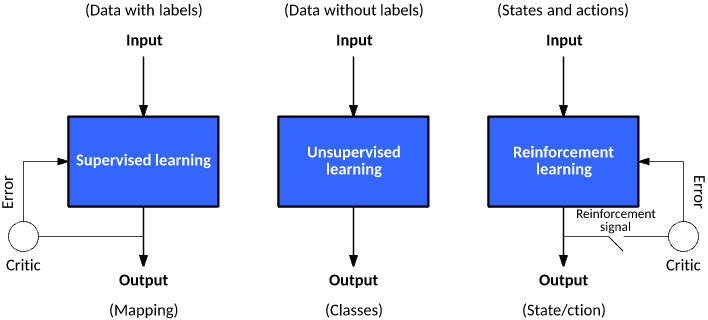
\includegraphics[width=\linewidth]{figures/ml-techniques}
	\caption{Types of Machine learning (\cite{jones2017models})}
	\label{fig:ml-types}
\end{figure}

\subsection{Programming by Demonstration}\label{sssec:PbD}
PbD, also known as Learning from Demonstration or Imitation Learning, describes various techniques where the robot learns new behaviours from teacher demonstrations. 
Unlike ML solutions, Programming by Demonstration (PbD) (\cite{billard2016learning,argall2009survey}), learns from \textit{biased} data in the form of demonstrations provided by a human teacher.
PbD systems have been used in the industry for creating assembly programs. 
In recent years there has been significant work in PbD to move from pure imitation to intelligent systems that learn flexible task executions. 
PbD systems may learn task descriptions from interpreted data to adapt the learned task to changing environments.

The user can choose to provide positive or negative examples (\cite{grollman2012robot}), to allow the robot to learn more efficiently by reducing the search space for possible solutions.
Positive examples are demonstration data showing what the robot should do and what it can learn directly from, i.e. where an action changes predicates.
Negative examples are what the robot should avoid but should help it to generalise faster by eliminating bad solutions from the search space, i.e. when an action fails because its preconditions are not satisfied.
However, \cite{walsh2010efficient} noted his Ph.D. thesis that negative examples are highly uninformative as the learner cannot determine the reason for the failure, while positive examples provide very useful information because a superset of the literals that belong to the precondition is identified.

%In contrast to reinforcement learning techniques, where the policy is learned from arbitrarily positive and negative experience, PbD approaches derive the policy from a dataset of selected examples.
%The robot derives a policy in various ways (\sect{subsec:Deriving a policy}). 

\subsubsection{Interaction Modalities}
There are different ways for a teacher to provide demonstration data, depending on the amount of data provided at a time (incremental vs. batch learning) and the different interaction modalities (voice, vision, and touch) to transfer the data to the robot.

\cite{profanter2015analysis} evaluated four input modalities (touch, gesture, speech, 3D tracking device) and showed that users preferred touch and gesture input and that speech input was the least preferred modality.

Natural language is the most intuitive way for humans to communicate instructions but may need some form of clarification and learning system in order to work efficiently. 
Instructive systems that use voice recognition to command robots to carry out tasks provide the user with a high-level control to program the action sequence by commanding sub-actions that robots have already been programmed (Forbes et al. 2015).
Instructive systems use voice recognition to command robots to carry out tasks while performing a demonstration.
Voice recognition is also used in PbD systems during demonstrations to activate in-built actions such as opening gripper or save end-effector poses (\cite{alexandrova2014robot}).

The teacher can also demonstrate the action using their own hands, while the robot observes the motion (\cite{kuniyoshi1994learning}).
Gestures can be used to direct the attention of the robot for indicating objects in a scene to which the instructions apply.
Demonstrations can also be provided by kinesthetically moving the robot's joints, allowing the robot to go through the action execution.
A multi-modal communication including information from vision, gesture and voice sources can be used to clarify instructions to the robot, for example mentioning ``that table" and gesturing the relevant object.


\section{End-user Involvement}\label{sssec:End-User Involvement}
There are different levels of end-user involvement in robot programming, such as writing and organising the execution code, providing biased or unbiased data, and defining reward functions. 
Table \ref{tab:enduserinvolvement} shows user involvement tasks for different programming methods, together with estimated effort (\eg time), and expertise required.
In this case we consider experts as users who have received formal training or experience in the stated programming method, \eg programming language or RL/DL-related concepts.
\cite{kormushev2013reinforcement} draws a comparison of the same main robot teaching approaches and compares computational complexity with difficulty for the teacher.

\begin{table}[ht]
	\centering
	\label{tab:enduserinvolvement}
	\begin{tabular}{llcc}
		\textbf{End-user task} & \textbf{Programming}   & \textbf{Effort} & \textbf{Expert} \\
		\textbf{}& \textbf{method}   & \textbf{ required} & \textbf{ required} \\ \hline
		Write code manually    & Text-based programming       & high                          & yes                      \\
		Organise code sequence & Visual programming           & moderately high               & no                       \\
		Provide complete data  & Deep learning (DL)               & moderate                      & yes                      \\
		Provide partial data   & Programming by demonstration (PbD) & moderately low                & no                       \\
		Define reward function & Reinforcement learning (RL)      & moderately low                & yes                     
	\end{tabular}
\caption{End-user involvement for common robot programming approaches}
\end{table}

Text-based programming, Deep learning and Reinforcement learning solutions require experts to construct the code, provide data or a reward function. Visual programming provides a simpler solution for end-users without programming experience, but still requires a logical understanding of the constructed program flow. Programming by demonstration provides a more intuitive low-effort solution as the robot, where the only difficulty lies in providing correct examples to the robot.


%\section{Robot Programming in Industrial Environments}\label{subsec:RP in Industrial Enviroments}
%The deployment of robots in industrial environments introduces additional constraints to the robot programming process, such as limited resources, time constraints, limited programming expertise, product-specific tasks.
%\cite{pan2012recent} give an overview of three main robot programming methods for industrial robots: offline programming, online programming, and using Augmented Reality. 
%
%\subsection{Offline Programming}\label{sssec:Offline Programming}
%Offline Programming (OLP) is based on 3D CAD data that models the complete robot work cell and lets the user fine-tune the properties of the robot's movements before generating a program that can be downloaded to the robot. 
%It is more efficient when programming complex systems with large volumes and more reliable compared to online programming. 
%As it requires a great amount of programming effort and a long delivery time, it requires high programming overhead and is not efficient for the development of smaller product volumes or customised software.
%
%Robot designers and users have developed computational platforms for OLP systems in form of packages that allow secondary development for specific applications. 
%These OLP packages simulate not only robot trajectories and assembly tasks, but can also model interactions of several manufacturing processes, resources and product maintenance issues. 
%Almost every robot manufacturer has its own OLP software. 
%There exist also generic OLP software that are more flexible for hardware from different manufacturers.
%
%Current OLP systems do not provide functions for the complete OLP process but include steps that need to be created manually. 
%Due to the high costs of OLP systems, their use is not cost-efficient for small to medium-sized enterprises.
%
%\subsection{Online Programming}\label{sssec:Online Programming}
%In online programming methods the robot program commands the robot to move through a recorded sequence of end-effector postures which form a complete task. 
%The postures are recorded using the teach pendant to manually move the end-effector to the desired position and orientation of the task. 
%Due to its simplicity, intuitiveness, and low programming skill requirement, this method is widely used. 
%However, it is only suitable for programming applications with uncomplicated processes and work pieces with simple geometry. 
%Once the program has been generated, it is difficult to make further amendments.
%
%\subsection{Augmented Reality}\label{sssec:Augmented Reality}
%The use of augmented reality (AR) is a revolutionary concept where computer-generated 3D objects are blended onto a real world scene to enhance the user's interaction with the real world (\cite{pettersen2003augmented}). 
%Robot programming using AR allows offline programming to be performed without the need to model the workpiece in the virtual environment (\cite{pan2012recent}). 
%It can eliminate technical difficulties faced by OLP techniques such as the calibration between the virtual and the real world.
